\documentclass{article}

% Math packages
\usepackage{amsthm, amssymb, enumitem}

% Margins settings
\usepackage[margin=1.2in]{geometry}

% Bracket notation (quantum computing/information)
\usepackage{tikz}
\usetikzlibrary{quantikz}
\usepackage{braket}

% Spacing
\usepackage{parskip}
\usepackage{centernot}

% Required for inserting images
\usepackage{graphicx}
\graphicspath{{./Figures/}}

% Hyperlinks
\usepackage[colorlinks=true, allcolors=blue]{hyperref}

% Header
\usepackage{fancyhdr}
\pagestyle{fancy}
\lhead{November 11th, 2024}
\chead{Optimization for Data Science}
\rhead{University of Waterloo}

% Custom commands
\newcommand{\R}{\mathbb{R}}             % real numbers
\newcommand{\M}{\mathcal{M}}            % set of matrices
\newcommand{\E}{\text{E}}               % expectation
\newcommand{\x}{\vec{x}}                % vector x
\newcommand{\y}{\vec{y}}                % vector y
\newcommand{\z}{\vec{z}}                % vector z
\newcommand{\dom}{\text{dom}}           % domain
\newcommand{\relint}{\text{relint}}     % relative interior
\newcommand{\ds}{\displaystyle}
\newcommand{\indep}{\perp\!\!\!\perp}

\newcommand{\rl}[1]{\left(#1\right)}

\setlength\parindent{0pt}

\title{CO 673/CS 794 - Optimization for Data Science\\Lecture 18 Notes}
\author{University of Waterloo}
\date{November 11th, 2024, 11h30-12h50 in MC 2054}

\begin{document}

\maketitle

\section{Administration}

\begin{itemize}
    \item Problem set 5 due Friday, November 15th, at 19h00
\end{itemize}

Addressing Piazza posts:
\begin{itemize}
    \item Numbering starts at 1,
    \item Ambiguous `$t$' in PS5 Q4. One meaning was for time, the other was the parameter to the prox function.
\end{itemize}

\section{Proximal Gradient Descent}

Recall the problem under consideration:
\[
    \min_{\x}\rl{\left\{f(\x) \psi(\x)\right\}}
\]
where $f$ is $L$-smooth and convex and $\dom(f) = \R^n$, and $\psi$ is a proper, convex, and closed "proximable"

PGD main iteration:
\begin{align*}
    \x_{k + 1} &= \text{prox}_(\psi/L)(\x_k - \frac{1}{L} \nabla f(\x_k)) \\
    &\overset{\text{(a)}}{=} \text{argmin}_{\z}\rl{\left\{\frac{\psi(\z)}{L} + \frac{1}{2}\|\x_k - \frac{1}{L} \nabla f(\x_k) - \z\|^2\right\}} \\
    &\overset{\text{(b)}}{=} \text{argmin}_{\z} \rl{\left\{\frac{\psi}{L} + \frac{1}{2} \|\x_k - \z\|^2 - \frac{1}{L}\nabla f(\x_k)^\top(\x_k - \z) + \underbrace{\frac{1}{2L^2}\|\nabla f(\x_k)\|^2}_{\indep \z}\right\}} \\
    &\overset{\text{(c)}}{=} \text{argmin}_{\z} \rl{\left\{\frac{\psi(\z)}{L} + \frac{1}{2}\|\x_k - \z\|^2 - \frac{1}{L}\nabla f(\x_k)^\top(\x_k - \z)\right\}} \\
    &\overset{\text{(d)}}{=} \text{argmin}_{\z} \rl{\left\{\psi(\z) + \frac{L}{2}\|\x_k - \z\|^2 - \nabla f(\x_k)^\top(\x_k - \z)\right\}} \\
    &\overset{\text{(e)}}{=} \text{argmin}_{\z} \rl{\left\{\psi(\z) + \underbrace{\frac{L}{2}\|\z - \x_k\|^2 + \nabla f(\x_k)^\top(\z - \x_k) + f(\x_k)}_{\overline{f}(\z)}\right\}}
\end{align*}
where:
\begin{enumerate}[label=(\alph*)]
    \item definition of prox
    \item partly expand norm
    \item minimizer unchanged by additive term
    \item minimizer unchanged by positive rescaling
    \item additive term
\end{enumerate}
Observe that $\overline{f}(\z)$ is a variant of a Taylor approximation about $\x_k$ for $f(\z)$.

% Taylor approximation table

\textbf{Theorem.} $\forall \z \in \R^n$, $\overline{f}(\z) \geq f(\z)$ (quadratic term is an overestimator).

\begin{proof}
    Restatement of the standard inequality tht characterizes $L$-smoothness.
\end{proof}

Why not use the true Taylor quadratic term in PGD in place of $\frac{L}{2}\|\z - \x_k\|^2$?

Problem: Evaluation of argmin on each iteration is much more complicated even for $\psi(\x) = \gamma \|\x\|_1$.

PGD is a particular instance of \textit{Operator splitting}
\begin{align*}
    \x &\mapsto \vec{x} - \frac{\nabla f(\x)}{L} \\
    \x &\mapsto \text{prox}_{\psi/L}(\x)
\end{align*}
both examples of ``monotone operators''.

PGD is also called ``Forward-backward splitting''.

\section{Projected Gradient Descent (Chapter 7)}

Projected gradient descent is a special case of proximal gradient descent in which $\psi(\x) = I_\Omega(\x)$, $\Omega \subset \R^n$ is closed, convex, and non-empty.

Recall:
\[
    I_\Omega(\x) = \begin{cases}
        0, & \x \in \Omega \\
        \infty, & \x \notin \Omega
    \end{cases}
\]
Hence,
\[
\min_{\x}\rl{\{f(\x) + I_\Omega(\x)\}} \quad \text{same as} \quad \min_{\x}\rl{\{f(\x)\}}, \text{ s.t. } \x \in \Omega
\]

Projected gradient descent is a useful algorithm if there is an efficient algorithm for $\text{prox}_{I_\Omega}$.

Recall:
\begin{align*}
    \text{prox}_{I_\Omega}(\x) &= \text{argmin}_{\z} \rl{\left\{I_\Omega(\z) + \frac{1}{2}\|\z - \x\|^2\right\}} \\
    &= \text{argmin}_{\z}\rl{\left\{\frac{1}{2}\|\z - \x\|^2 : \z \in \Omega\right\}} \\
    &= \text{proj}_{\Omega}(\x)
\end{align*}

Example 1.

$\Omega = \overline{B}_r\rl{\vec{0}}$, and so
\[
    \text{proj}_{\Omega}(\x) = \begin{cases}
        \x, & \|\x\| \leq r \\
        r\frac{\x}{\|\x\|}, & \|\x\| > r
    \end{cases}
\]

E.g. $n = 2$:
\begin{center}
    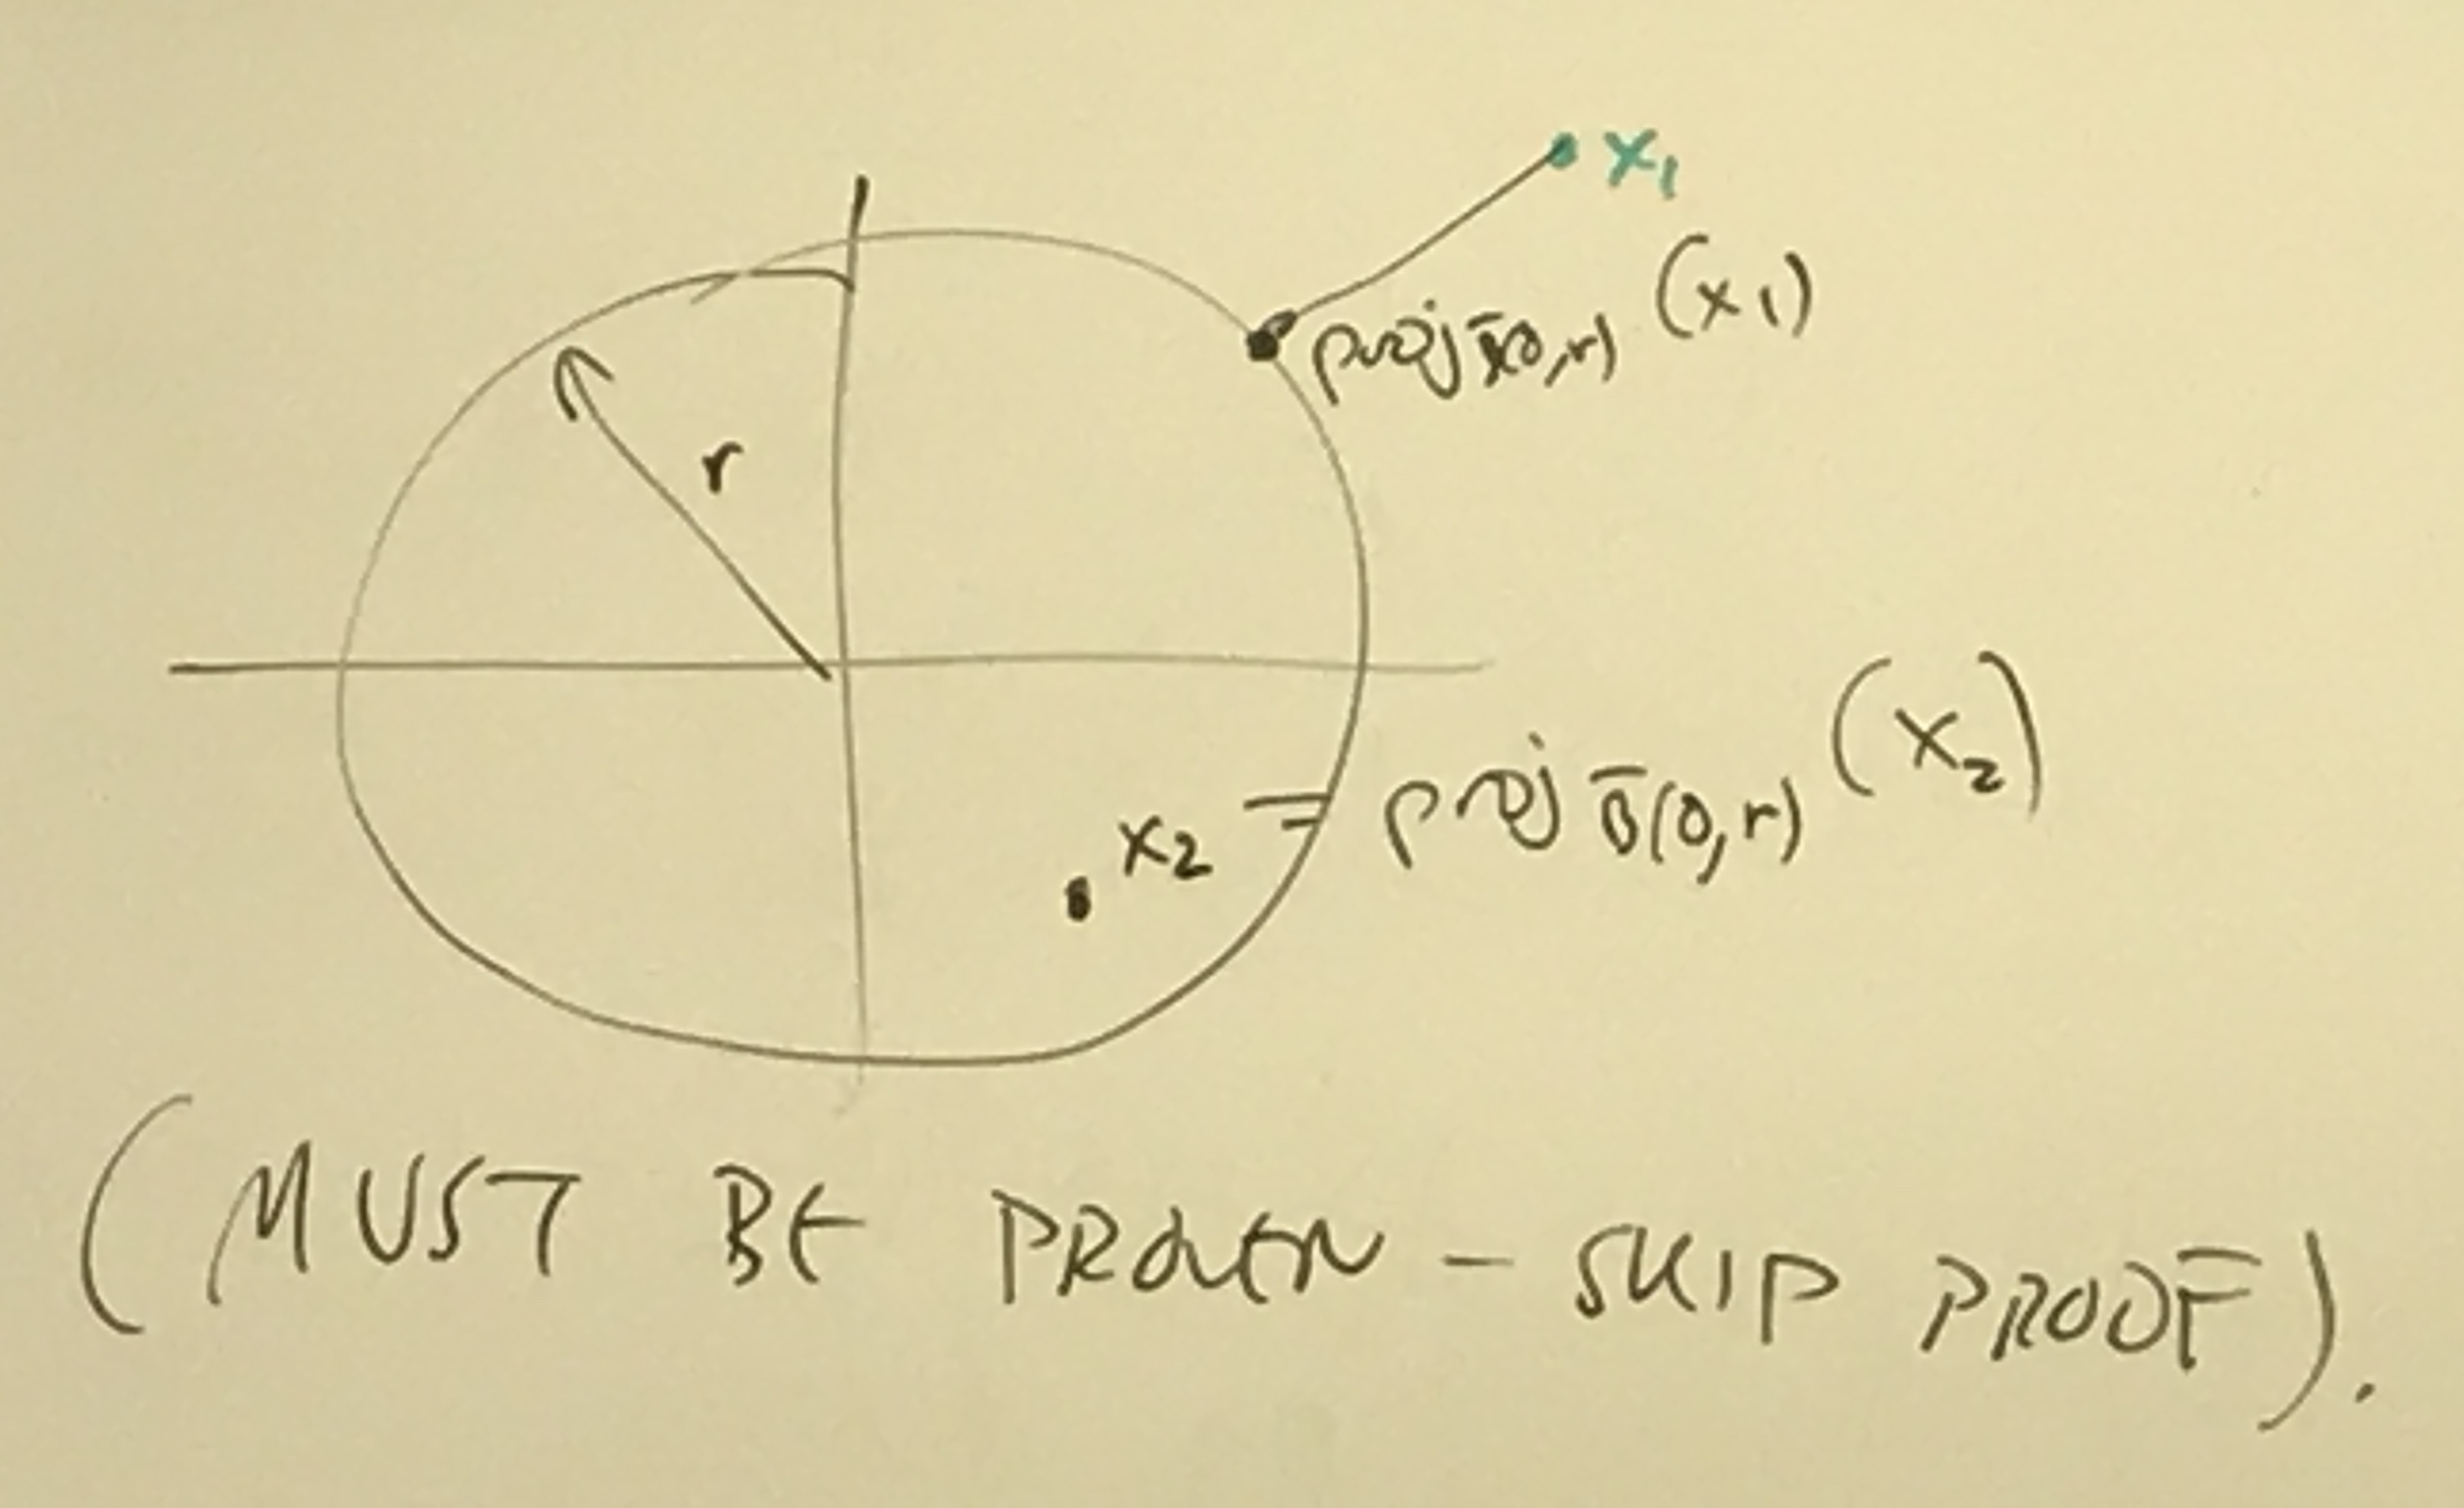
\includegraphics[scale=0.1]{projection.JPG}
\end{center}

Example 2.

$\Omega = \{\x \in \R^n : A\x = \vec{b}\}$ where $A \in \M_{m,\, n}(\R)$ and $\vec{b} \in \R^m$. Assume we have $\x_0$ such that $A\x_0 = \vec{b}$.

Find matrix $U$ with orthonormal columns that form a basis for $\null(A)$ (SVD; QR-factorization)

Say $U \in \M_{n,\, p}$. If the rows of $A$ are independent, then $p = n - m$.

$U^\top U = I$ (orthonormal columns)

$A\x = \vec{b} \iff \exists \vec{w} \in \R^p$ such that $\x = \x_0 + U\vec{w}$.

\textbf{Theorem.} If $A$, $\vec{b}$, $\x_0$, $U$, $\Omega$ are defined as above. Then,
\[
    \text{proj}_{\Omega}(\x) = x_0 + UU^\top(\x - \x_0)
\]

\begin{proof}
    \begin{align*}
        &\min_{\z} \rl{\left\{\frac{1}{2}\|\z - \x\|^2 : A\z = \vec{b}\right\}} \intertext{Change of variable: $z = \x_0 + U\vec{w}$}
        = &\min_{\vec{w}} \rl{\left\{\frac{1}{2}\|U\vec{w} + \x_0 - \x\|^2\right\}} \\
        = &\min_{\vec{w}} \rl{\left\{\frac{1}{2}\vec{w}^\top \underbrace{U^\top U}_{=\, I}\vec{w} + (\x_0 - \x)^\top U\vec{w} + \text{constant}\right\}} \\
        = &\min_{\vec{w}}\rl{\left\{\frac{1}{2}\|\vec{w} + U^\top(\x_0 - \x)\|^2 + \text{different constant}\right\}}
    \end{align*}
    Take $\vec{w} = -U^\top(\x_0 - \x)$ to minimize. So,
    \[
        \z = \x_0 + UU^\top(\x - \x_0)
    \]
\end{proof}

Example 3. ``Hyperrectangle'':
\[
    \bigtimes_{j = 1}^{j = n} [a_j;\; b_j]
\]

Example 4. ``Standard simplex'':
\[
    \{\x : \vec{1}^\top \x = 1,\, \x \geq \vec{0}\}
\]

One step of projected gradient descent:
\[
    \x_{k + 1} := \text{proj}_{\Omega}\rl{\x_k - \frac{1}{L}\nabla f(\x_k)}
\]
Nexterov acceleration is also applicable to projected gradient descent.

\section{Duality}

Leading to kernel amchines and alternating direction method of multipliers (ADMM). Partly covered in Chapter 10

Nonlinear programming (NLP, not ``natural language processing''):
\[
    \min_{\x}\rl{f_0(\x)} \text{ s.t. } f_1(\x) \leq 0,\, \ldots,\, f_m(\x) \leq 0,\, A\x = \vec{b}
\]
We later specialize to constraint programming (CP).

Let $\Omega := \{\x : \forall k \in \{1,\, \ldots,\, m\},\, f_k(\x) \leq 0 \wedge A\x = b\}$ where $f_0,\, \ldots,\, f_m \colon \R^n \to \R \cup \{\infty\}$, $A \in \M_{p,\, n}(\R)$, and $b \in \R^p$.

The Lagrangian is
\[
    L\rl{\x,\, \vec{\lambda},\, \vec{\mu}} = f_0(\x) + \sum_{k = 1}^{k = m}\lambda_k f_k(\x) + \vec{\mu}^\top(A\x - \vec{b})
\]
where $\vec{\lambda} \in \R^m$ and $\vec{\mu} \in \R^p$, the Lagrange multipliers.

\textbf{Theorem.} Assume that NLP has a solution $\x^*$. Then, by definition
\begin{align*}
    f_0(\x^*) &= \min_{\x}\rl{\{f_0(\x) : \x \in \Omega\}} \\
    &\overset{\text{(a)}}{=} \min_{\x \in \R^n}\rl{\left\{\max_{\vec{\lambda} \geq \vec{0},\, \vec{\mu}}\rl{\{L\rl{\x,\, \vec{\lambda},\, \vec{\mu}}\}}\right\}}
\end{align*}
Equality (a) must be proved. This is the saddle-point formulation of NLP.

\begin{proof}
    From the saddle-point formulation, we have the two following cases:

    Case 1. $\x \notin \Omega$:
    \begin{itemize}
        \item Case 1a.

        $\exists k$ such that $f_k(\x) > 0$. Take $\vec{\mu} = \vec{0}$ and $\vec{\lambda} = t\ket{k - 1}$ where $\ket{k - 1}$ is column $k$ of identity matrix $I$. $t \to \infty \implies L\rl{\x,\, \vec{\lambda},\, \vec{\mu}} \to \infty$ so inner max of Lagrangian is $\infty$. Thus, $\x$ cannot be a minimizer.

        \item Case 1b. $A\x \neq \vec{b}$.

        Take $\vec{\lambda} = \vec{0}$ and $\vec{\mu} = t(A\x - \vec{b})$. The last term of $L\rl{\x,\, \vec{\lambda},\, \vec{\mu}}$ is $t\|A\x - \vec{b}\|^2$. The inner max is again $\infty$, so $\x$ cannot solve outer min.
    \end{itemize}

    Case 2. $\x \in \Omega$:
    \[
        L\rl{\x,\, \vec{\lambda},\, \vec{\mu}} = \underbrace{\sum_{k = 1}^{k = m} \underbrace{\lambda_k}_{\geq\, 0} \underbrace{f_k(\x)}_{\leq\, 0}}_{\leq\, 0} + \underbrace{\vec{\mu}^\top\underbrace{(A\x - \vec{b})}_{=\, 0}}_{=\, 0} \leq f_0(\x)
    \]

    If $\vec{\lambda} = \vec{0}$, $\vec{\mu} = \vec{0}$, then $L\rl{\x,\, \vec{\lambda},\, \vec{\mu}} = f_0(\x)$. So, inner max evaluates to $f_0(\x)$.

    This proves the theorem.
\end{proof}

\textbf{Theorem.} (Weak duality)
\[
    \min_{\x}\rl{\left\{\max_{\vec{\lambda} \geq \vec{0},\, \vec{\mu}}\rl{\left\{L\rl{\x,\, \vec{\lambda},\, \vec{\mu}}\right\}}\right\}} \geq \max_{\vec{\lambda} \geq \vec{0},\, \vec{\mu}}\rl{\left\{\min_{\x}\rl{\left\{L\rl{\x,\, \vec{\lambda},\, \vec{\mu}}\right\}}\right\}}
\]

\begin{proof}
    Given $\x_1$, $\vec{\lambda}_1 \geq \vec{0}$, $\vec{\mu}$, we have that
    \[
        L\rl{\x_1,\, \vec{\lambda}_1,\, \vec{\mu}_1} \geq \min_{\x}\rl{\left\{L\rl{\x,\, \vec{\lambda}_1,\, \vec{\mu}_1}\right\}},
    \]
    i.e., $\x_1$ is a candidate. This holds for arbitrary $\vec{\lambda}_1 \geq \vec{0}$, $\vec{\mu}$, so take the maximum over them.

    \[
        \max_{\vec{\lambda} \geq \vec{0},\, \vec{\mu}}\rl{\left\{L\rl{\x,\, \vec{\lambda},\, \vec{\mu}}\right\}} \geq \max_{\vec{\lambda} \geq \vec{0},\, \vec{\mu}}\rl{\left\{\min_{\x}\rl{\left\{L\rl{\x,\, \vec{\lambda},\, \vec{\mu}}\right\}}\right\}}
    \]
    Since true $\forall \x_1$, it is also true given the minimum over $\x_1$. Thus,
    \[
        \min_{\x}\rl{\left\{\max_{\vec{\lambda} \geq \vec{0},\, \vec{\mu}}\rl{\left\{L\rl{\x,\, \vec{\lambda},\, \vec{\mu}}\right\}}\right\}} \geq \max_{\vec{\lambda} \geq \vec{0},\, \vec{\mu}}\rl{\left\{\min_{\x}\rl{\left\{L\rl{\x,\, \vec{\lambda},\, \vec{\mu}}\right\}}\right\}}
    \]
\end{proof}

Strong duality means $\exists \x^*$, $\vec{\lambda}^* \geq \vec{0}$, and $\vec{\mu}^*$ such that the left-hand side evaluated at $\x^*$ equals the right-hand side evaluated at $\vec{\lambda}^*$ and $\vec{\mu}^*$.

Notation:
\[
    g(\vec{\lambda},\, \vec{\mu}) := \min_{\x}\rl{\left\{L\rl{\x,\, \vec{\lambda},\, \vec{\mu}}\right\}}
\]
This is called the dual objective function.

The Dual problem is:
\[
    \max_{\vec{\lambda} \geq \vec{0},\, \vec{\mu}} \rl{\left\{g(\vec{\lambda},\, \vec{\mu})\right\}}
\]
Strong duality: $\exists \x^* \in \Omega$, $\vec{\lambda}^* \in \R^m$ where $\vec{\lambda} \geq \vec{0}$, and $\vec{\mu} \in \R^p$ such that $f_0\rl{\x_0} = g\rl{\vec{\lambda}^*,\, \vec{\mu}^*}$ (sometimes holds).

Weak duality:
\[
    \forall \x \in \Omega,\, \forall \vec{\lambda} \geq \vec{0},\, \forall \vec{\mu},\, f_0\rl{\x} \geq g\rl{\vec{\lambda},\, \vec{\mu}}
\]
(always holds).

\end{document}
